\chapter{Computer Graphics}

    \section{Math Engine}
        \subsection{vector.cpp}
            the Vector3 class supports operations such as addition, subtraction, dot product, and cross product, enabling users to perform complex calculations with ease.
        \subsection{random.cpp}
            Generating true-randomness is one of the biggest computer science challenges. 

            In my project i needed a way the user to be able to get a "insert formal specs here for non-deterministic random" vector3 and color variable. 

            Lukily, i have stumbled upon this random-generator function and was able to implement it. Now, in the framework there is a function that returns a different each call random variable and also the seed is randomized so it differes between individual launches of the application. 
    \section{Renderer Engine}
        \subsection{primitives}
            OpenGL and WebGL are quite similar. P5.js is built on top of WebGL and offers the end-user (besides many more) a set of convenient functions for simple tasks like drawing the background, drawing a square, a circle, choosing stroke width and color.
        
            besides these functions i have thought of implementing classes for each of the base geometrical shapes. This implementation will come in handy when integrating with the game engine stuff (see chapter3:Game Development, section GameObjects). For example, each renderer component will use one of the primitive classes (square, circle, box, sphere) to display itself on the screen.
            
        \subsection{Transformations}
            As we've already mentioned in the mathematics chapter, transformations are a big deal when dealing with game development. They basically give fluidity. Also, they can be a tough challenge to overcome, especially because it requires the mathematical framework to be able to do complex calculations and as quickly as possible. 

            This topic is brought up multiple times in this paper and in this chapter we will focus on the specifics on how primitives transform.
            
            types of transformation:
            \begin{itemize}
                \item translation
                \item rotation
                \item scaling
                \item skewing
                \item warping
                \item ...
            \end{itemize}

            fun fact: did u know that u can achieve a rotation by doing multiple skew transformations in a row?
        \subsection{color.cpp}
    \section{Collision Detection}



% \section{Titlul secțiunii 1}

% \begin{figure}
%     \centering
%     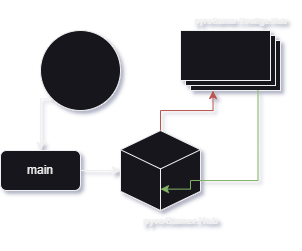
\includegraphics[width=0.5\linewidth]{chapters/pyroGamerHub.png}
%     \caption{Enter Caption}
%     \label{fig:enter-label}
% \end{figure}

% Id donec ultrices tincidunt arcu non sodales neque. Integer eget aliquet nibh praesent. Euismod in pellentesque massa placerat duis ultricies lacus sed. Mauris ultrices eros in cursus turpis massa. Integer quis auctor elit sed vulputate mi. Nibh ipsum consequat nisl vel pretium lectus quam id leo. Vel elit scelerisque mauris pellentesque pulvinar pellentesque. Suscipit tellus mauris a diam maecenas. Ultrices eros in cursus turpis massa tincidunt. Tristique senectus et netus et malesuada fames ac turpis egestas. Suspendisse interdum consectetur libero id faucibus nisl tincidunt eget. Sed risus pretium quam vulputate dignissim suspendisse in. Donec adipiscing tristique risus nec feugiat in fermentum posuere. A lacus vestibulum sed arcu non odio euismod lacinia at.

% \section{Titlul secțiunii 2}

% Pellentesque pulvinar pellentesque habitant morbi tristique senectus et. Ornare suspendisse sed nisi lacus sed viverra tellus in hac. Non sodales neque sodales ut etiam sit. In hendrerit gravida rutrum quisque non. Diam quam nulla porttitor massa id neque aliquam. Diam sit amet nisl suscipit adipiscing bibendum est ultricies integer. Cras fermentum odio eu feugiat pretium nibh ipsum. Egestas integer eget aliquet nibh praesent tristique magna. Porttitor eget dolor morbi non arcu risus quis varius quam. Gravida rutrum quisque non tellus orci. Diam volutpat commodo sed egestas egestas.